%!TEX root = ../dissertation.tex
\chapter{FAIR principles comparison}
\label{AppendixA}
% Please add the following required packages to your document preamble:
% \usepackage{multirow}


{\setlength\LTleft{-2cm}
\setlength\LTright{-2cm}
\scriptsize
% \footnotesize
\begin{longtable}{@{\extracolsep{\fill}} p{6cm}   p{6cm}  p{6cm}}
\textbf{FAIR Guiding Principles (2016)}    & \textbf{Towards FAIR Principles for research software (2020)}            & \textbf{FAIR4RS Principles (2022)}\\
\hline
\hline
\multicolumn{2}{l}{Findable} &  \\
\hline
The first step in (re)using data is to find them. Metadata and data should be easy to find for both humans and computers. Machine-readable metadata are essential for automatic discovery of datasets and services, so this is an essential component of the FAIRification process. & The main concern of findability for research software is to ensure software can be identified unambiguously when looking for it using common search strategies. & Software, and its associated metadata, is easy for both humans and machines to find. \\
\hline
F1. (Meta)data are assigned a globally unique and persistent identifier & F1. Software and its associated metadata have a global, unique and persistent identifier for each released version. & F1. Software is assigned a globally unique and persistent identifier. \\
 &  & F1.1. Components of the software representing levels of granularity are assigned distinct identifiers. \\
 &  & F1.2. Different versions of the software are assigned distinct identifiers. \\
\hline
F2. Data are described with rich metadata (defined by R1 below) & F2. Software is described with rich metadata. & F2. Software is described with rich metadata. \\
\hline
F3. Metadata clearly and explicitly include the identifier of the data they describe & F3. Metadata clearly and explicitly include identifiers for all the versions of the software it describes. & F3. Metadata clearly and explicitly include the identifier of the software they describe. \\
\hline
F4. (Meta)data are registered or indexed in a searchable resource & F4. Software and its associated metadata are included in a searchable software registry. & F4. Metadata are FAIR, searchable and indexable. \\
\hline
\multicolumn{2}{l}{A. Accessible} &  \\
\hline
Once the user finds the required data, she/he needs to know how can they be accessed, possibly including authentication and authorisation. & Accessibility translates into retrievability {[}...{]} however, we found mere retrievability not enough. In order for anyone to use any research software, a working version of the software needs to be available. & Software, and its metadata, is retrievable via standardized protocols. \\
\hline
A1. (Meta)data are retrievable by their identifier using a standardized communications protocol & A1. Software and its associated metadata are accessible by their identifier using a standardized communications protocol. & A1. Software is retrievable by its identifier using a standardized communications protocol. \\
\hline
A1.1. The protocol is open, free, and universally implementable & A1.1. The protocol is open, free, and universally implementable. & A1.1. The protocol is open, free, and universally implementable. \\
\hline
A1.2. The protocol allows for an authentication and authorization procedure, where necessary & A1.2. The protocol allows for an authentication and authorization procedure, where necessary. & A1.2. The protocol allows for an authentication and authorization procedure, where necessary. \\
\hline
A2. Metadata are accessible, even when the data are no longer available & A2. Software metadata are accessible, even when the software is no longer available. & A2. Metadata are accessible, even when the software is no longer available. \\
\hline
\multicolumn{2}{l}{I. Interoperable} &  \\
\hline
The data usually needs to be integrated with other data. In addition, the data need to interoperate with applications or workflows for analysis, storage, and processing. & Interoperability for research software can be understood in two dimensions: as part of workflows (horizontal dimension) and as stack of digital objects that need to work together at compilation and execution times (vertical dimension) & Software interoperates with other software by exchanging data and/or metadata, and/or through interaction via application programming interfaces (APIs), described through standards. \\
\hline
I1. (Meta)data use a formal, accessible, shared, and broadly applicable language for knowledge representation. & I1. Software and its associated metadata use a formal, accessible, shared and broadly applicable language to facilitate machine readability and data exchange. & I1. Software reads, writes and exchanges data in a way that meets domain-relevant community standards \\
\hline
I2. (Meta)data use vocabularies that follow FAIR principles & I2.1. Software and its associated metadata are formally described using controlled vocabularies that follow the FAIR principles. & Now split between F4 and I1. \\
 & I2.2. Software use and produce data in types and formats that are formally described using controlled vocabularies that follow the FAIR principles. &  \\
\hline
I3. (Meta)data include qualified references to other (meta)data &  & I2. Software includes qualified references to other objects. \\
\hline
 & I4S. Software dependencies are documented and mechanisms to access them exist. &  \\
\hline
\multicolumn{2}{l}{R. Reusable} &  \\
\hline
The ultimate goal of FAIR is to optimize the reuse of data. To achieve this, metadata and data should be well-described so that they can be replicated and/or combined in different settings. & Reusability in the context of software has many dimensions. At its core, reusability aims for someone to be able to reuse software reproducibly. & Software is both usable (can be executed) and reusable (can be understood, modified, built upon, or incorporated into other software). \\
\hline
R1. (Meta)data are richly described with a plurality of accurate and relevant attributes & R1. Software and its associated metadata are richly described with a plurality of accurate and relevant attributes. & R1. Software is described with a plurality of accurate and relevant attributes. \\
\hline
R1.1. (Meta)data are released with a clear and accessible data usage license & R1.1. Software and its associated metadata have independent, clear and accessible usage licenses compatible with the software dependencies. & R1.1. Software is given a clear and accessible license. \\
\hline
R1.2. (Meta)data are associated with detailed provenance & R1.2. Software metadata include detailed provenance, detail level should be community agreed. & R1.2. Software is associated with detailed provenance. \\
\hline
R1.3. (Meta)data meet domain-relevant community standards & R1.3. Software metadata and documentation meet domain-relevant community standards. & R3. Software meets domain-relevant community standards. \\
\hline
 &  & R2. Software includes qualified references to other software.
\hline
% \caption{FAIR principles\label{long}}\\
%  \label{tab:activitiy}
\end{longtable}}



\chapter{Repository type labels}
\label{AppendixB}


{\setlength\LTleft{-1.25cm}
\setlength\LTright{-1cm}
% \scriptsize
\begin{longtable}{@{\extracolsep{\fill}} p{2cm}   p{14.5cm}  p{1.5cm}}
\textbf{Label} & \textbf{Description} &  \textbf{Research software?} \\
\hline
\hline
Research Software & Is the tool used for research or was it produced during research? If it is installable (has setup file, is a package, Docker installation) it counts as Research Software. GUIs and (shiny) apps also   count as Research Software. If there is no documentation but code structure implies reusability,   it is still counted as Research Software, even if the author describes it as a "simple   script". Parts used by other software that are reusable also count as   Research Software. & Yes \\
\hline
Rscript & Generally things that are only   for reproducibility of specific analyses or workflows, not reusability   directly. Scripts that need (heavy) modification to be used for other   purposes that the original intent. Additionally, scripts for benchmarking,   testing or showcasing of research software. Queries like SPARQL scripts are   also considered research scripts. & Yes \\
\hline
RSWIP & Research Software that is currently WIP or in   alpha/experimental phase. Based on available information within a repository   or corresponding documentation. Incomplete abandoned software is also   considered RSWIP. Releases in R with version number less than 1.0 considered   RSWIP according to best practices:   https://lifecycle.r-lib.org/articles/stages.html\#experimental & Yes \\
\hline
Empty & Includes placeholder   repositories that have not much more than a few lines of text or a license. & No \\
\hline
Non-RS & Other kind of software, for   example for simplifying or automating workflows that were not clearly   developed during research process. Software and scripts created for learning   or other purposes not directly related to research. & No \\
\hline
Rdata & Repositories with only research   data. If they contain research software or scripts, they will be classified   as such. & No \\
\hline
Workshop & This includes course and   exercise material, tutorials, workshops. & No \\
\hline
Docs & This includes notes, summaries,   documentation, lists, presentations, ontologies, websites, guidelines, LaTeX   files, lecture slides, project management (projects tab), publication PDFs,   vignettes, books, and anything else falling into this category. & No \\
\hline
Template & Code, LaTeX or documentation   templates/boilerplates that are not created during the research process   according to our used definition. & No \\
\hline
Student work & Bachelor and master thesis   related work, student coursework etc.; Actual research projects by students   conducted under supervision (e.g. scientific internships) are not part of   this category. Thesis work published on organizational accounts are counted as   Research Software/Rscripts. & No \\
\hline
OtherRS & Research Software from researchers that were   developed at other institutions. & No \\
\hline
Irrelevant & Test/dummy/Toy/Demo/course   project/non-scientific code challenge repositories. Also includes other types   of repositories, e.g. for storing artwork, data dumps of misc. projects,   storage for configuration files, schemas, stylings, themes, moved or deleted repositories. & No

% \caption{FAIR variables description \label{tab:var}}
\end{longtable}}


\chapter{Further user plots}
\label{app:user_plots}
\vspace{-1.1cm}
\begin{figure}[htb!]
\centerline{
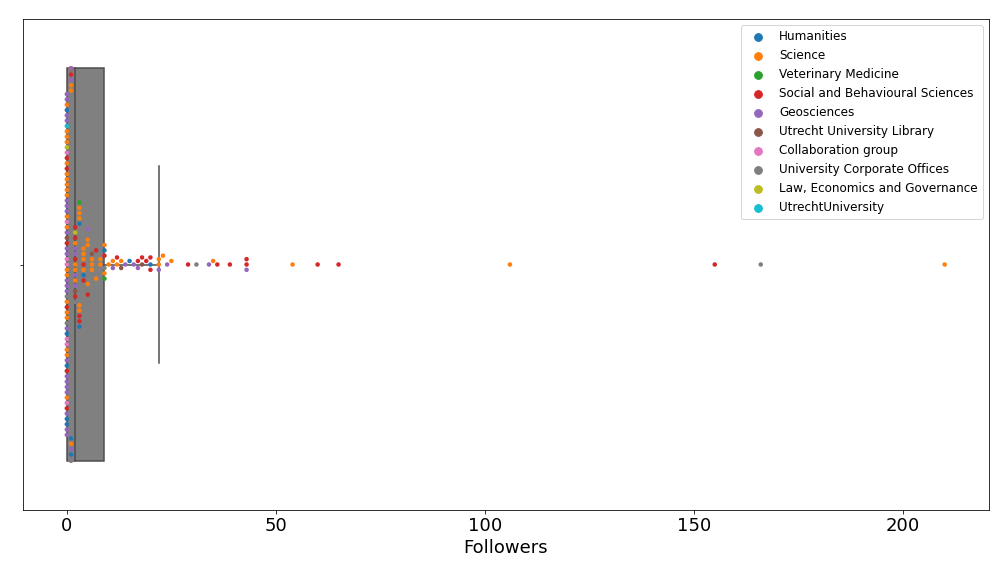
\includegraphics[scale=0.48]{figures_results/extra/user_followers.png}}
\caption{Number of followers of users per faculty.}
\vspace{-0.45cm}
\centerline{
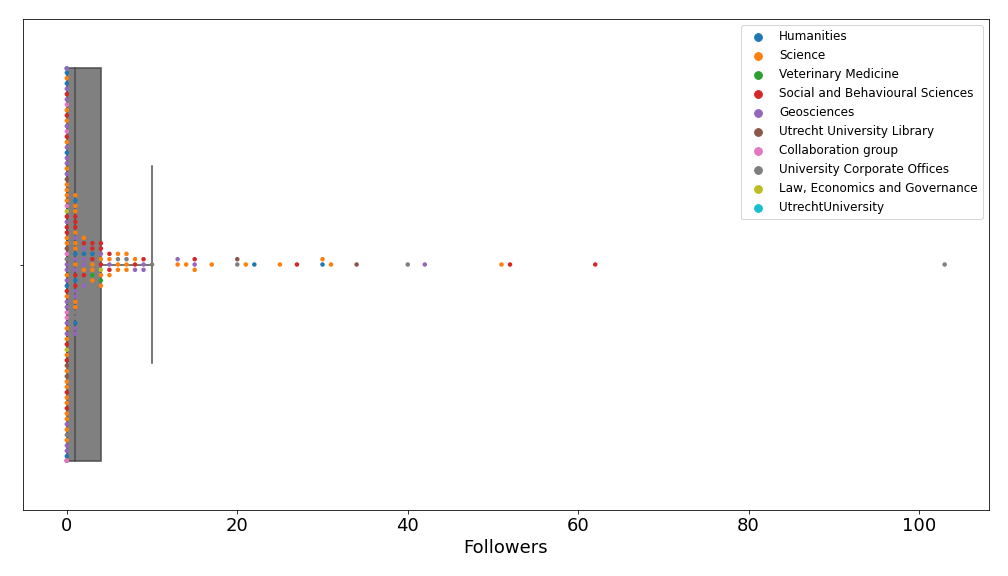
\includegraphics[scale=0.48]{figures_results/extra/user_following.png}}
\caption{Number of users a user is following per faculty.}

\end{figure}


\chapter{Further repository plots}
\label{app:repo_plots}

\begin{figure}[h!]
\centerline{
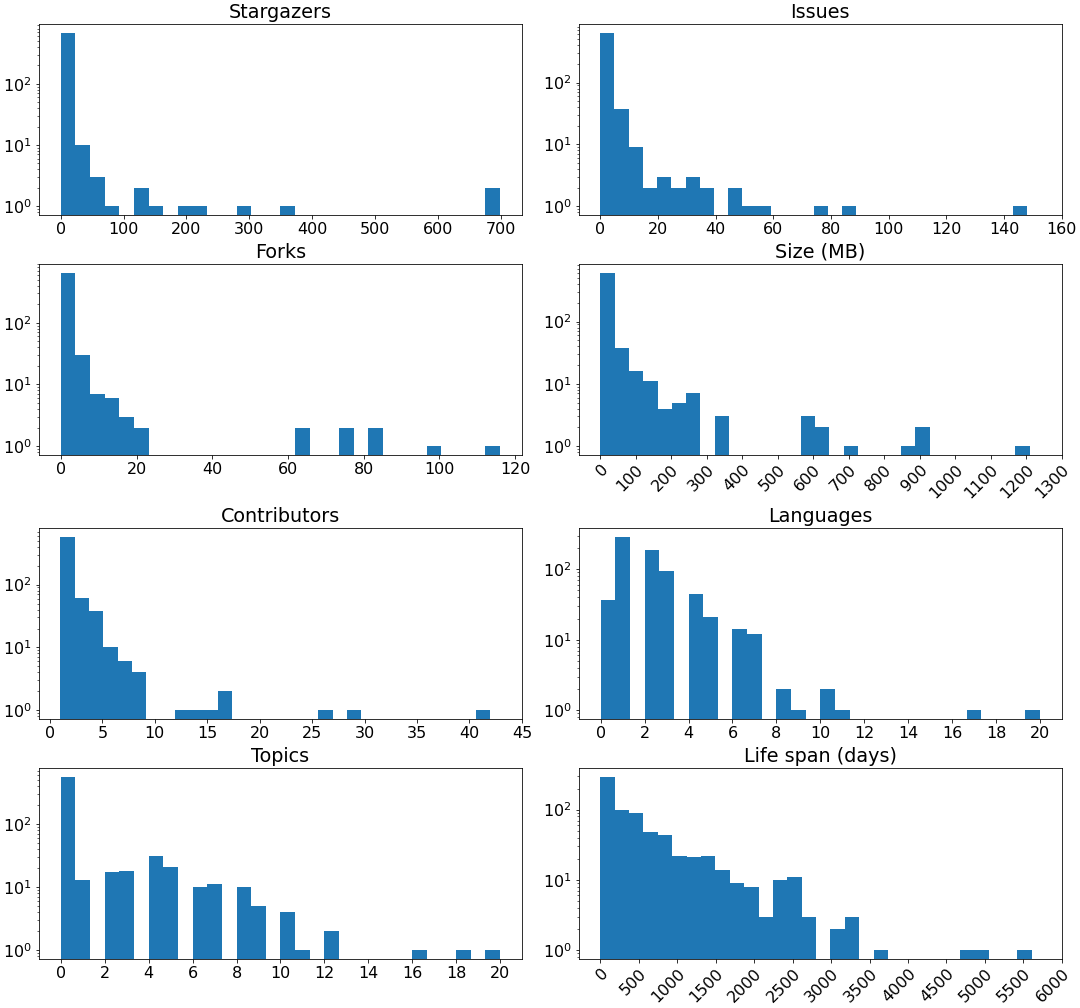
\includegraphics[scale=0.5]{figures_results/extra/stats_histograms_rs_only.png}}
\caption{Histograms for metrics that are considered research software. The y-axis is log-scaled.
\label{fig:stats_histograms_rs_only}}
\end{figure}


\begin{figure}[h!]
\centerline{
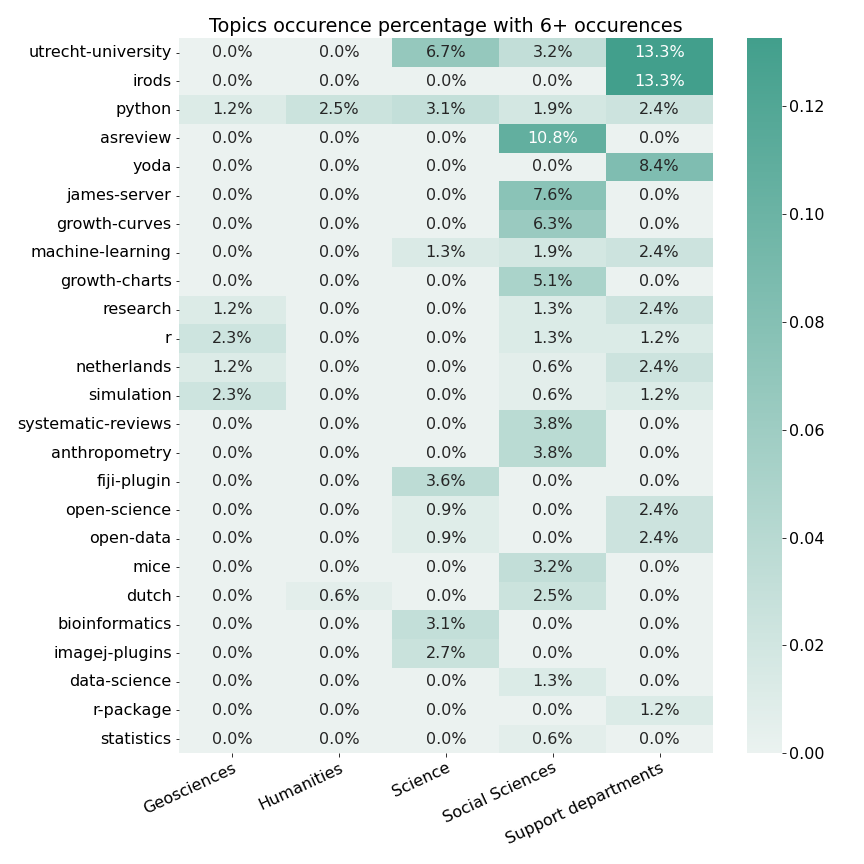
\includegraphics[scale=0.6]{figures_results/extra/heatmap_topics_percentage.png}}
\caption{Topics percentage for each faculty. Only topics that occurred more than 6 times were included.
\label{fig:heatmap_topics_percentage}}
\end{figure}


\chapter{Descriptive statistics per faculty}
\label{app:stats_faculty}

\begin{table}
\centering
\caption{Descriptive statistics of numeric variables for Geosciences}
\label{tab:Geosciences}
\begin{tabular}{lcccccccc}
\toprule
{} &  Stargazers &  Issues &  Forks &    Size &  Contributors &  Languages &  Topics &  Life span \\
\midrule
Minimum         &        0.00 &    0.00 &   0.00 &    0.00 &          1.00 &       0.00 &    0.00 &       0.00 \\
25th percentile &        0.00 &    0.00 &   0.00 &    0.02 &          1.00 &       1.00 &    0.00 &       5.25 \\
Mean            &        2.84 &    3.02 &   1.49 &   16.96 &          1.22 &       2.19 &    0.62 &     467.95 \\
Median          &        0.00 &    0.00 &   0.00 &    0.12 &          1.00 &       2.00 &    0.00 &     266.50 \\
75th percentile &        1.00 &    0.00 &   0.75 &    5.98 &          1.00 &       3.00 &    0.00 &     656.00 \\
Maximum         &       80.00 &  148.00 &  62.00 &  263.95 &          4.00 &      20.00 &   10.00 &    3623.00 \\
Skewness        &        5.70 &    7.05 &   8.07 &    3.67 &          2.88 &       4.42 &    3.30 &       2.33 \\
Kurtosis        &       33.76 &   51.33 &  69.78 &   14.09 &          8.77 &      26.72 &   10.97 &       5.99 \\
\bottomrule
\end{tabular}
\end{table}

\begin{table}
\centering
\caption{Descriptive statistics of numeric variables for Humanities}
\label{tab:Humanities}
\begin{tabular}{lcccccccc}
\toprule
{} &  Stargazers &  Issues &  Forks &  Size (MB) &  Contributors &  Languages &  Topics &  Life span (days) \\
\midrule
Minimum         &        0.00 &    0.00 &   0.00 &       0.00 &          1.00 &       0.00 &    0.00 &              0.00 \\
25th percentile &        0.00 &    0.00 &   0.00 &       0.08 &          1.00 &       1.00 &    0.00 &             39.25 \\
Mean            &        0.58 &    2.92 &   0.18 &       9.52 &          1.79 &       2.36 &    0.25 &            591.39 \\
Median          &        0.00 &    0.00 &   0.00 &       0.42 &          1.00 &       2.00 &    0.00 &            430.00 \\
75th percentile &        0.00 &    2.00 &   0.00 &       4.92 &          2.00 &       3.00 &    0.00 &            816.50 \\
Maximum         &       11.00 &   77.00 &   3.00 &     205.65 &          9.00 &       7.00 &   11.00 &           2796.00 \\
Skewness        &        4.34 &    5.54 &   3.43 &       4.56 &          2.58 &       1.02 &    6.60 &              1.38 \\
Kurtosis        &       21.09 &   35.84 &  12.59 &      28.83 &          7.79 &       0.45 &   48.36 &              1.23 \\
\bottomrule
\end{tabular}
\end{table}

\begin{table}
\centering
\caption{Descriptive statistics of numeric variables for Science}
\label{tab:Science}
\begin{tabular}{lcccccccc}
\toprule
{} &  Stargazers &  Issues &  Forks &    Size &  Contributors &  Languages &  Topics &  Life span \\
\midrule
Minimum         &        0.00 &     0.0 &   0.00 &    0.00 &          1.00 &       0.00 &    0.00 &       0.00 \\
25th percentile &        0.00 &     0.0 &   0.00 &    0.11 &          1.00 &       1.00 &    0.00 &      38.00 \\
Mean            &        8.71 &     1.3 &   2.42 &   38.85 &          2.08 &       2.17 &    1.17 &     590.09 \\
Median          &        1.00 &     0.0 &   0.00 &    1.17 &          1.00 &       2.00 &    0.00 &     278.00 \\
75th percentile &        3.00 &     0.0 &   1.00 &   11.75 &          2.00 &       3.00 &    0.00 &     764.00 \\
Maximum         &      699.00 &    53.0 &  97.00 &  927.14 &         42.00 &      17.00 &   20.00 &    5609.00 \\
Skewness        &       11.19 &     7.1 &   7.87 &    5.26 &          9.36 &       3.39 &    3.11 &       2.77 \\
Kurtosis        &      141.37 &    56.8 &  66.58 &   32.71 &        110.80 &      17.78 &   12.14 &       9.64 \\
\bottomrule
\end{tabular}
\end{table}

\begin{table}
\centering
\caption{Descriptive statistics of numeric variables for Social Sciences}
\label{tab:Social_Sciences}
\begin{tabular}{lcccccccc}
\toprule
{} &  Stargazers &  Issues &  Forks &  Size (MB) &  Contributors &  Languages &  Topics &  Life span (days) \\
\midrule
Minimum         &        0.00 &    0.00 &   0.00 &       0.00 &          1.00 &       0.00 &    0.00 &              0.00 \\
25th percentile &        0.00 &    0.00 &   0.00 &       0.13 &          1.00 &       1.00 &    0.00 &             34.00 \\
Mean            &        6.78 &    1.36 &   1.99 &      34.96 &          1.99 &       1.77 &    1.37 &            514.22 \\
Median          &        0.00 &    0.00 &   0.00 &       1.45 &          1.00 &       1.00 &    0.00 &            336.50 \\
75th percentile &        1.75 &    0.00 &   1.00 &       9.53 &          2.00 &       2.00 &    2.00 &            759.25 \\
Maximum         &      350.00 &   36.00 &  84.00 &     870.33 &         29.00 &       7.00 &   18.00 &           3337.00 \\
Skewness        &        8.30 &    4.91 &   7.93 &       5.09 &          6.92 &       1.75 &    2.66 &              1.86 \\
Kurtosis        &       71.01 &   26.28 &  65.80 &      27.67 &         53.17 &       3.64 &   10.23 &              4.03 \\
\bottomrule
\end{tabular}
\end{table}

\begin{table}
\centering
\caption{Descriptive statistics of numeric variables for Support departments}
\label{tab:Support_departments}
\begin{tabular}{lcccccccc}
\toprule
{} &  Stargazers &  Issues &   Forks &  Size (MB) &  Contributors &  Languages &  Topics &  Life span (days) \\
\midrule
Minimum         &        0.00 &    0.00 &    0.00 &       0.00 &          1.00 &       0.00 &    0.00 &              0.00 \\
25th percentile &        0.00 &    0.00 &    0.00 &       0.07 &          1.00 &       1.00 &    0.00 &             74.00 \\
Mean            &       12.16 &    2.07 &    3.46 &      29.54 &          2.46 &       2.01 &    1.83 &            452.88 \\
Median          &        0.00 &    0.00 &    0.00 &       0.56 &          2.00 &       1.00 &    0.00 &            256.00 \\
75th percentile &        2.00 &    1.50 &    1.00 &       3.13 &          3.00 &       3.00 &    3.00 &            548.50 \\
Maximum         &      694.00 &   49.00 &  116.00 &    1209.65 &         17.00 &       7.00 &   12.00 &           2375.00 \\
Skewness        &        8.55 &    6.42 &    6.43 &       7.04 &          3.84 &       1.35 &    1.78 &              1.75 \\
Kurtosis        &       75.39 &   49.14 &   43.42 &      52.86 &         16.16 &       1.89 &    3.08 &              2.48 \\
\bottomrule
\end{tabular}
\end{table}
